\documentclass[assignment04_Solutions]{subfiles}

\IfSubStr{\jobname}{\detokenize{Solutions}}{\toggletrue{solutions}}{\togglefalse{solutions}}

\fancypagestyle{firstpage}

{\rhead{Assignment 4 \linebreak \textit{Version: \today}}}

\title{Assignment 4: Sequence Learning and Maximum Likelihood Estimation}
\author{Machine Learning}
\date{Fall 2019}

\invalidatemargin

\begin{document}

\maketitle
\thispagestyle{firstpage}


\begin{learningobjectives}
\bi
\item Understand the idea of maximum likelihood estimation and apply it to the Na\"ive Bayes model.
\item Learn the basic ideas of sequence prediction and approach the problem using bigrams.
\item Learn about word embeddings.
\ei
\end{learningobjectives}

\section{Placeholder for Companion Notebook}
TODO

\section{Word Embeddings}
As we've seen in this assignment and the previous one, treating each word as a unique entity can result in missed opportunities for learning.  For instance, when predicting the sentiment of a movie review, if we don't know that the words \emph{terrific} and \emph{fabulous} have similar meanings, we are going to need a lot of data to learn a good model of sentiment classification.

Word embeddings are one answer to this problem.  A word embeddings takes each word and maps it into a vector space where words that have similar meanings are are nearby in the vector space (e.g., they have a small Euclidean distance between them).  Methods have been proposed that allow one to learn these word embeddings from giant collections of raw, unlabeled text.  Thus, we can develop high quality, numerical representations of the meanings of various words using unlabeled data, and then use a smaller collection of labeled data (for instance, movie reviews with corresponding sentiment values) along with these representations to learn the task at hand.

\begin{externalresources}[(45 minutes)]
We'd like you to get the basic idea of word embeddings so you can dig into some important issues regarding bias in machine learning.  We think these resources are written at a level where you can get some important details without this becoming unmanageable.

\bi
\item Watch \href{https://www.youtube.com/watch?v=QyrUentbkvw}{Jordan Boyd-Graber's video on word2vec} (after 15:00 he goes into a connection to the singular value decomposition (SVD), that you shouldn't worry about).
\item If you prefer (or would also like) a written resource, consider \href{https://www.analyticsvidhya.com/blog/2017/06/word-embeddings-count-word2veec/}{An Intuitive Understanding of Word Embeddings: From Count Vectors to Word2Vec}.  This resource builds up to word2vec from simpler methods, which you can skip if you'd like.  The most directly relevant path through the content is to read: Intro,  What are Word Embeddings?, Prediction based Embedding, Word Embeddings use case scenarios.
\ei
\end{externalresources}

\subsection{Bias in Word Embeddings}

\begin{externalresources}[(45 minutes)]
\bi
\item Read \href{https://developers.googleblog.com/2018/04/text-embedding-models-contain-bias.html}{Text Embedding Models Contain Bias. Here's Why That Matters}
\item \textbf{(Optional)} if you are up for a denser read and want to spend more time on this read \href{https://papers.nips.cc/paper/6228-man-is-to-computer-programmer-as-woman-is-to-homemaker-debiasing-word-embeddings.pdf}{Man is to Computer Programmer as Woman is to Homemaker? Debiasing Word Embeddings} (\textbf{to be clear, you will not be able to read this article in 45 minutes})
\ei
\end{externalresources}

\section{Maximum Likelihood Parameter Estimation for Discrete Models}
In assignment 2, you met the Na\"ive Bayes model.  As a motivating example, we presented a Bayesian Network (BN) for the Titanic Dataset that modeled three features (\emph{is male}, \emph{is young}, and \emph{fare class}) being generated by whether or not the passenger survived.  Here is the BN corresponding to this model.

\begin{center}
\includegraphics[width=0.6\linewidth]{../02/figures/titanicbn}
\end{center}

In assignment 2, we described how we determined the parameters in the conditional probability tables.
\begin{quote}
``The probabilities in this BN were computed by looking at the training set and counting the appropriate passengers that fell into each category.  For instance, to compute $p(\mathcal{Y}|\mathcal{S})$ since $p(\mathcal{Y}|\mathcal{S}) = \frac{p(\mathcal{Y}, \mathcal{S})}{p(\mathcal{S})}$, we can approximate this probability by counting the number of passengers under 5 who survived and dividing by the total number who survived (note that there are some subtle and important modifications to this method of fitting these probabilities that we'll discuss in the next assignment).  This process was repeated for each conditional probability.  Since we assume that all of the features are conditionally independent given the output ($\mathcal{S}$ in this case), this process is done independently for each feature.''
\end{quote}

In the assignment 3 companion notebook on sentiment analysis, we employed very similar logic (for instance counting the number of reviews that had positive sentiment and a particular word and dividing it by the number of reviews with positive sentiment).

While these methods of parameter fitting (hopefully) seem logical, it helps to be rigorous about \emph{why} these are the right probabilities to fit given the training data.  In this section, we'll go over the math behind determining these probabilities.  The goal will be to provide a general outline of a process for fitting parameters of a BN.  We'll do so by analyzing the Na\"ive Bayes model in particular to help you get the ``recipe'' for how this works.

\subsection{Formalizing the Problem}
We can think of the numbers in the conditional probability tables as the parameters of our Bayesian Network.  In order to compute sensible values for those parameters, we're going to choose the parameters values that agree as closely as possible with a set of training data.  At a conceptual level this strategy should feel pretty familiar.  In the last module, we did this again and again by tuning model parameters to accurately predict the training outputs as a function of the training inputs (last module the parameters were typically weights of a neural network or a logistic regression model).

Suppose we are given $n$ training data points $\mathbf{x_1}, \mathbf{x_2}, \ldots, \mathbf{x_n}$.  In the case of the titanic dataset $\mathbf{x_i}$ would be a four-dimensional vector consisting of whether the passenger survived ($\mathcal{S}$), the passenger's fare class ($\mathcal{C}$), whether the passenger was male ($\mathcal{M}$), and whether the passenger was under the age of 5 ($\mathcal{Y}$).  Further, suppose our model is parameterized by parameters $\mathbf{\Theta}$, which provide the necessary information to compute the probability of any input $\mathbf{x}$.  In other words, our model can compute $p(\mathbf{x_i} | \mathbf{\Theta})$ for any of the training points (or any other possible input for that matter).

\begin{understandingcheck}
In the case of the Titanic model, what would the parameters $\mathbf{\Theta}$ represent? (check solutions for the answer).
\begin{boxedsolution}
The parameters in this case would represent all of the entries in the conditional probability tables in the BN.  For example, the parameters would encode $p(\mathcal{S})$, $p(\mathcal{M}|\mathcal{S})$, etc.
\end{boxedsolution}
\end{understandingcheck}

Given our model of $p(\mathbf{x_i}|\mathbf{\Theta})$, we would now like to figure out the best parameters, $\mathbf{\Theta}^\star$ based on our training data.  To do this, we can use the technique of maximum likelihood estimation (MLE).  The maximum likelihood estimate of the parameters is given by the following formula.

\begin{align}
\mathbf{\Theta^\star} &= \argmax_{\mathbf{\Theta}} p(\mathbf{x_1}, \mathbf{x_2}, \ldots \mathbf{x_n} | \mathbf{\Theta}) \label{eq:mle}
\end{align}

This equation is known as maximum likelihood estimation because: (a) it involves a maximization and (b) it is a likelihood (probability of data given a hypothesis or model).  Intuitively, Equation~\ref{eq:mle} captures the idea that we should choose the model parameters that makes the observed training data as likely as possible under our model.

\subsection{Simplifications to Equation~\ref{eq:mle}}

It may seem that computing the probability in Equation~\ref{eq:mle} would be quite difficult.   While in some cases it can be, there are some simplifying assumptions that we can apply to make our lives easier.  One of the most common assumptions is that the training points are conditionally independent given $\mathbf{\Theta}$ (that is $X_i \condindep X_j~|~\mathbf{\Theta}$ for all $i \neq j$).  This is known as the \href{https://en.wikipedia.org/wiki/Independent_and_identically_distributed_random_variables}{independently and identically distributed (i.i.d.) assumption}.

\begin{understandingcheck}
Make sure you have a good conceptual sense of what the i.i.d. assumption is all about.  Perhaps a good thing to think through would be why $X_i$ and $X_j$ are \emph{not} independent (they are only conditionally independent given $\mathbf{\Theta}$.
\end{understandingcheck}

If we apply the i.i.d. assumption to Equation~\ref{eq:mle}, we derive the following equation.

\begin{align}
\mathbf{\Theta^\star} &= \argmax_{\mathbf{\Theta}} p(\mathbf{x_1} |  \mathbf{\Theta}) p(\mathbf{x_2} | \mathbf{\Theta}) \ldots p(\mathbf{x_n} | \mathbf{\Theta}) \label{eq:mleiid}
\end{align}

To make things even easier, we can apply a log without changing the $\argmax$.  This works because $\log$ is a monotonic (continuously increasing) function, so $\argmax_x f(x) = \argmax_x \log  f(x)$ for any monotonic function $f$.


\begin{align}
\mathbf{\Theta^\star} &= \argmax_{\mathbf{\Theta}} \log \left ( p(\mathbf{x_1} |  \mathbf{\Theta}) p(\mathbf{x_2} | \mathbf{\Theta}) \ldots p(\mathbf{x_n} | \mathbf{\Theta})  \right) \nonumber \\
&=  \argmax_{\mathbf{\Theta}} \sum_{i=1}^n \log p(\mathbf{x_i} |  \mathbf{\Theta})  \label{eq:mleiidlog}
\end{align}

The importance of applying the log might not be apparent yet, but it actually did some useful work for us.  Specifically, it broke apart our probability into multiple components (one for each data point).  We can now optimize the sum of a bunch of terms rather than the product  of a bunch of terms (the former turns out to be much easier).  We'll see how this plays out in the next section.

\subsection{Maximum Likelihood Estimation for Na\"ive Bayes}

In this section you'll be applying the technique of MLE to the Na\"ive Bayes algorithm.



\vspace{1em}
\begin{exercise}[(60 minutes)]
The BN for the Na\"ive Bayes model is shown below.

\begin{center}
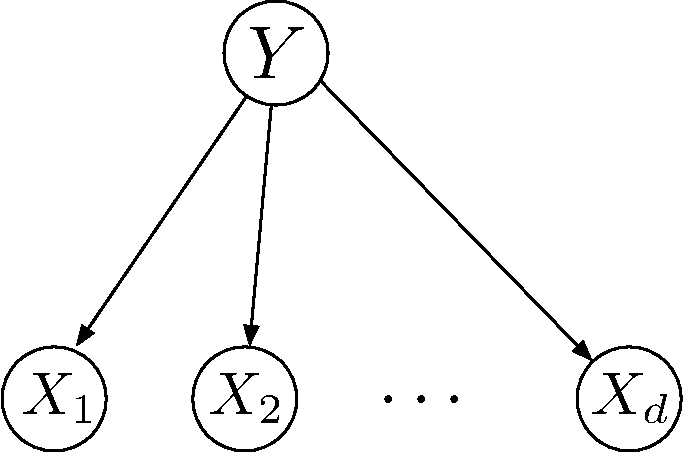
\includegraphics[width=0.3\linewidth]{figures/naivebayesgm}
\end{center}

In this BN, the variable $\mathcal{Y}$ represents some category of interest (e.g., survive versus not survive), and $X_1, X_2, \ldots, X_d$ represent various features of a data point (e.g., age, sex, fare class).  The rules of d-separation tell us that $X_i \condindep X_j~|~Y$ for all $i \neq j$.  For simplicity, we'll assume that $Y$ takes on values from the set $\{1, 2, \ldots c \}$ and each $X_i$ takes on values from the set $\{1, 2, \ldots, r\}$.  Extending your work to the case where each of the random variables takes values from some other discrete set is straightforward.

%Suppose we want to apply the technique of maximum likelihood estimation to the Na\"ive Bayes model.  For training data you are given a training set of input output pairs as $\left (\mathbf{x_1}, y_1 \right),  \left (\mathbf{x_2}, y_2 \right), \ldots, \left (\mathbf{x_n}, y_n \right)$.  Each $\mathbf{x_i}$ represents a $d$ dimensional vector that corresponds to the values of the random variables, $X$, in the BN (e.g., the $j$ the random variable in the BN $X_j$ for the $i$th data point would equal $x_{i,j}$).  Each $y_i$ represents a value for the random variable $Y$ in the bn (e.g., the random variable $Y$ for the $i$th data point would equal $y_i$).

\bes
\item Equation~\ref{eq:mleiidlog} can be written for this model as
\begin{align}
\mathbf{\Theta^\star} &= \argmax_{\Theta} \sum_{i=1}^n \log p(X_1 = x_{i,1}, X_2 = x_{i,2}, \ldots, X_d = x_{i,d}, Y = y_i | \mathbf{\Theta}) \enspace . \label{eq:nbmle}
\end{align}
Using the concept of d-separation on the BN graph for Na\"ive Bayes (the figure above), simplify Equation~\ref{eq:mleiidlog}.  Hint: you'll want to break apart the big joint probability (the probability of all of the $X_i$'s and $Y$ using conditional independence). %SWM: I changed this to the above equation instead of the equation shown in part b.

Warning: spoiler alert if you look at part b.
\begin{boxedsolution}
We know that each of the variables in a BN is conditionally independent given its parents.  We can use this result to write the joint probability of all of our random variables the $X$'s and $Y$ in terms of the probability of each conditioned on its parents.
\begin{align}
\mathbf{\Theta^\star} &= \argmax_{\mathbf{\Theta}} \sum_{i=1}^n  \left ( \log p(Y = y_i | \mathbf{\Theta})  + \sum_{j=1}^d \log p(X_j = x_{i,j} | Y = y_i,  \mathbf{\Theta}) \right ) \enspace . 
\end{align}
\end{boxedsolution}

\item The answer to part (a) is given here to help setup the next part of this question.

\begin{align}
\mathbf{\Theta^\star} &= \argmax_{\mathbf{\Theta}} \sum_{i=1}^n  \left ( \log p(Y = y_i  | \mathbf{\Theta})  + \sum_{j=1}^d \log p(X_j = x_{i,j} | Y = y_i,  \mathbf{\Theta}) \right ) \enspace . \label{eq:nbmlesolved}
\end{align}

Suppose, $\mathbf{\Theta}$ consists of the following parameters.
\bi
\item $\Theta(1), \Theta(2), \ldots, \Theta(c)$ represent the prior probability that $y$ takes on a particular value (e.g., $\Theta(i) = p(Y = i)$).  Note that in order for $\Theta(1), \ldots, \Theta(c)$ to represent a valid probability mass function $\sum_{i=1}^c \Theta(i) = 1$.
\item $\Theta_{j}(k | i)$ represents the conditional probability that feature $X_j = k$ given $Y = i$.  That is $\Theta_{j}(k | j) = p(X_j = k | Y = i)$.  In order for the $\Theta_j(k|i)$'s to represent valid PMFs, $\sum_{k=1}^{r} \Theta_{j}(k | j) = 1$ for all $j$ and $i$.
\ei

Suppose that $\mbox{ycount}(i)$ represents the number of training points where $y = i$ (i.e., $\mbox{ycount}(i) = \sum_{j=1}^n \mathbb{I} \left [y_j = i \right]$ where $\mathbb{I}$ is the indicator function, which returns 1 if the condition is true and 0 otherwise).

Suppose that $\mbox{xcount}_j(k|i)$ represents the number of training points where $x_j = k$ and $y = i$ (i.e., $\mbox{xcount}_j (k|i) = \sum_{u=1}^n \mathbb{I} \left [ x_{u, j} = k, y_j = i \right ]$).

Rewrite Equation~\ref{eq:nbmlesolved} in terms of the $\Theta(i)$'s, $\Theta_{j}(k|i)$'s, $\mbox{ycount}$'s, and $\mbox{xcount}$'s.  Hint: replace summations over the data points with summations over the possible values that the random variables can take on.

Warning: spoiler alert if you look at part c.
\begin{boxedsolution}
To help understand the logic of what we're going to do in this solution, consider the summation $\sum_{i=1}^n  \log p(Y = y_i  | \mathbf{\Theta})$.  The value of the term we are summing will depend on $\mathbf{\Theta}(y_i)$ (the probability that our model assigns to the $Y=y_i$.  Similarly, the term in the second part of the equation we are simplifying,  $\sum_{i=1}^n  \sum_{j=1}^d \log p(X_j = x_{i,j} | Y = y_i,  \mathbf{\Theta})$, only depends on $\mathbf{\Theta}_j(x_{i,j}~|~y_i)$.  Given these observations, we can rewrite the equation in the following way.

\begin{align}
\mathbf{\Theta^\star} &= \argmax_{\mathbf{\Theta}} \sum_{i=1}^n  \left ( \log  \mathbf{\Theta}(y_i)  + \sum_{j=1}^d \log \mathbf{\Theta}_j(x_{i,j}~|~y_i) \right ) \nonumber \\
&=  \argmax_{\mathbf{\Theta}} \left ( \sum_{i=1}^n \log  \mathbf{\Theta}(y_i) \right) + \left ( \sum_{i=1}^n  \sum_{j=1}^d \log \mathbf{\Theta}_j(x_{i,j}~|~y_i) \right)  &\mbox{break it apart to make it easier to deal with} \nonumber
\end{align}

We can further change these equations by removing the summations over the $n$ training points and instead summing over each of the possible values of $y_i$ (weighting by the count) and each possible combination of the values of $(y_i, x_{i,j})$ (again weighting by the count). We already defined the relevant counts above, so now we'll just substitute them into the equation.

\begin{align}
\mathbf{\Theta}^\star &= \argmax_{\mathbf{\Theta}} \left ( \sum_{i=1}^c \mbox{ycount}(i) \log \Theta(i)  \right) +  \left ( \sum_{j=1}^d \sum_{i=1}^c \sum_{k=1}^r \mbox{xcount}_j(k|i) \log \Theta_j(k|i) \right )
\end{align}
\end{boxedsolution}

\item The maximum likelihood equation for the model (the answer to part b) is as follows.
\begin{align}
\mathbf{\Theta}^\star &= \argmax_{\mathbf{\Theta}} \left ( \sum_{i=1}^c \mbox{ycount}(i) \log \Theta(i)  \right) +  \left ( \sum_{j=1}^d \sum_{i=1}^c \sum_{k=1}^r \mbox{xcount}_j(k|i) \log \Theta_j(k|i) \right ) \label{eq:mleparameterized}
\end{align}

Since each of the various parameters only affects particular terms in these summations, we can break the maximization over the entire parameters space $\mathbf{\Theta}$ into a bunch of separate maximization problems.  For example, the first summation in Equation~\ref{eq:mleparameterized} is only affected by $\Theta(1), \Theta(2), \ldots, \Theta(c)$, therefore
\begin{align}
\Theta^\star(1), \ldots, \Theta^\star(c)&= \argmax_{\Theta(1), \ldots, \Theta(c)}\sum_{i=1}^c \mbox{ycount}(i) \log \Theta(i) \enspace . \label{eq:qmarginals}
\end{align}

One thing to remember about this equation is that not all values of $\Theta(1), \ldots, \Theta(c)$ are permissible.  We know that these parameters have to specify a valid probability mass function, which requires that $\sum_{i=1}^c \Theta(i) = 1$ and each $\Theta(i) \geq 0$. In the language of numerical optimization, these equations are known as \emph{constraints}.

Additionally, for $i$ in the set $\{1, 2, \ldots, c\}$ and $j$ in the set $\{1, 2, \ldots, d\}$
\begin{align}
\Theta_j^\star(1|i), \ldots, \Theta^\star_j(r|i) &= \argmax_{\Theta_j(1|i), \ldots, \Theta_j(r|i)}\sum_{k=1}^r \mbox{xcount}_j(k|i) \log \Theta_j(k|i) \enspace . \label{eq:qconditionals}
\end{align}
For similar reasons to the ones we just stated for  $\Theta(1), \ldots, \Theta(c)$, Equation~\ref{eq:qconditionals} must satisfy $\sum_{k=1}^r \Theta_j(k|i) = 1$  and each $\Theta_j(k|i) \geq 0$ (the reason being, again, that these values must specify a valid PMF).

One way to derive the solution to these constrained optimization problems, is to use the technique of \href{http://tutorial.math.lamar.edu/Classes/CalcIII/LagrangeMultipliers.aspx}{Lagrange Multipliers}.  Here is \href{http://www.cs.columbia.edu/~mcollins/em.pdf}{a walkthrough of using this strategy to solve the equations for the Na\"ive Bayes algorithm} (the proof is in section 4.2).  Instead of having you prove this directly (do prove it if you feel inclined), let's take as given the following theorem.

Suppose $c_1, \ldots c_m$ represent non-negative constants ($c_i \geq 0)$.  Further, suppose $q_1, \ldots q_m$ represents a PMF ($q_i \geq 0$ and $\sum_{i=1}^m q_i = 1$).  If this is true then,

\begin{align}
q^\star_1, \ldots, q^\star_m &= \argmax_{q_1, \ldots, q_m} \sum_{i=1}^m c_i \log q_i \label{eq:multisetup} \\
q^\star_i &= \frac{c_i}{\sum_{j=1}^m c_j} \label{eq:multinomial}
\end{align}
These equation are pretty dense, so let's take a minute to unpack them.  Equation~\ref{eq:multisetup} is stating that our goal is to compute values of $q_1, \ldots q_m$ that maximize $\sum_{i=1}^m c_i \log q_i$.  We also require (but did not write explicitly in the equation) that $q_1, \ldots, q_m$ define a valid probability mass function ($q_i \geq 0$ and $\sum_{i=1}^m q_i = 1$).  Equation~\ref{eq:multinomial} states, without proof, the solution to Equation~\ref{eq:multisetup} (again, it's not too crazy to prove this if you would like to try).

Using the theorem above, find the optimal values of the parameters of the Na\"ive Bayes model.  In other words, compute $\Theta^\star(1), \ldots, \Theta^\star(c)$ and $\Theta_j^\star(1|i), \ldots, \Theta^\star_j(r|i)$ (for all appropriate values of $i$ and $j$).  Does the result match your intuitions about what the $\Theta$ values should be?

Hint: You should be able to pattern match Equation~\ref{eq:multinomial} to both Equation~\ref{eq:qmarginals} and Equation~\ref{eq:qconditionals}. 

\begin{boxedsolution}
Equation~\ref{eq:qmarginals} can be solved using Equation~\ref{eq:multinomial} in the following way.
\begin{align}
\Theta^\star(i) &= \frac{\mbox{ycount}(i)}{\sum_{j=1}^c \mbox{ycount}(j)}
\end{align}

Equation~\ref{eq:qconditionals} can be solved using Equation~\ref{eq:multinomial} in the following way.
\begin{align}
\Theta_j^\star(k|i) &= \frac{\mbox{xcount}_j(k|i)}{\sum_{u=1}^r \mbox{xcount}_j(u|i)}
\end{align}

The answers both seem logical since in the case of computing the $\Theta^\star(i)$ we just counted the number of training points that had $Y=i$ (this matches what we did in previous assignments).  In the case of computing $\Theta^\star_j(k|i)$ we calculated the proportion of training inputs where $X_j = k$ and divided by the sum of the number of training points that where $X_j$ took on some other value (the summation in the denominator should be the same as the total number of training points).
\end{boxedsolution}
\ees
\end{exercise}



\end{document}
